


\section{Installation and upgrade guide} \label{sec:install}

There are at least three methods of installing DiFX employed by its various users.
Ironically, these do not include some of the more common installation mechanisms such as those offered natively by various Linux distributions (e.g., {\tt .rpm} or {\tt .deb} files).
DiFX has many modules, some of which have dependencies that are not easily met or that are not needed.
Some modules have optional dependencies.
Finally, many folks may wish to have several versions installed at one time.
These considerations and the effort involved in overcoming some of them have led to the current situation where package-by-package compilation is the standard mechanism for installation.

The sections that follow document two of these methods.
First an install method using the {\tt difxbuild} script is described.
Then a more manual method is described.


\subsection{Installation with {\tt difxbuild}} \label{sec:installdifxbuild}


\subsubsection{Introduction}

This installation guide is based on the python program {\tt difxbuild}.
This program allows installation and management of multiple versions, each on multiple platforms, and associate setup scripts.
First some terminology: A {\em version} is a official numbered release of DiFX or an unofficial intermediate version drawn from the subversion repository.
Examples are the recent stable 2.1 release and the head of the development, called trunk.
Each {\em version} described here has a name.
The name for the two versions mentioned here are {\tt DIFX-2.1} and {\tt DIFX-DEVEL} respectively.
An {\em architecture} (or {\em arch} for short) is a computer type, usually defined by the instruction set of the CPU.
Currently {\tt difxbuild} explicitly knows about two architectures: {\tt x86\_64} for 64-bit Intel CPUs and {\tt i386} for 32-bit Intel CPUs.
The architecture of your machine can be determined on the command line with {\tt uname -p}.
Finally a {\em platform} is a particular configuration defined both by the {\em architecture} and the set of dependent software installed on it.
For example, if multiple Mark5 units with different software development kit (SDK) versions are being used, each would be a different {\em platform}.
For each DiFX installation there is a primary, or default, {\em platform} simply identified by the name of the {\em version}.
Each additional {\em platform} is assigned an additional name (which could be {\tt SDK8} and {\tt SDK9} for the Mark5 situation) and is identified by concatenating the version name, a hyphen, and the additional name (e.g., {\tt DIFX-2.1-SDK8}).

The installation process has a number of steps, including bootstrapping, source acquisition and autotooling, building (separately on each {\em platform}).
Any of these steps can be repeated if needed, however, in many cases it does not make sense to repeat a single step out of order, so following steps may need to be performed to be meaningful.

In the description below, each place where a command is to be typed into the computer, it is displayed after a $\longrightarrow$ .

\subsubsection{Assumptions}

To simplify the installation and eventual execution of DiFX, some assumptions are explicitly made:

\begin{enumerate}

\item It is assumed that before the DiFX installation is started that a fully usable Linux operating system is already running and a few bits of software are installed.
This specifically includes the Intel Integrated Performance Primitives (IPP) which must be directly acquired through Intel's web site.

\item It is assumed that all machines running DiFX cross mount the same filesystem, that the local name of the cross-mounted filesystem is the same on each machine, and that all parts of the DiFX installation will reside on such a partition.

\item It is assumed that during source acquisition steps the machine on which <code>difxbuild</code> is being invoked has access to the internet (specifically http and svn).

\item It is assumed here that {\tt bash} (or a compatible equivalent) is the shell used both by root and the user.
If this is not met, it is up to the user to make any needed procedural changes.

\end{enumerate}

\subsubsection{Installation Part 1}

Part 1 of installation deals with aspects of the installation that are specific to one {\em version} but all {\em architectures} and {\em platforms}.
For each new {\em version} of DiFX, these steps will be repeated.

\vspace{10pt}
\noindent
{\bf Bootstrapping:}

The bootstrapping step can start from a pristine computer (as long as the above assumptions are met) and will generate a skeleton DiFX environment from a rather simple input file.
This bootstrap input file consists of a few lines of ASCII text that describe in a minimal manner 
the intended parameters of the DiFX installation.
A complete description of such a file can be found in \S\ref{sec:bootstrapfile}.

Below is an example {\tt .bootstrap} file:

\begin{verbatim}
#-------------------------------------
# here are version-specific parameters
#-------------------------------------

# version of DiFX installed by this file
version = DIFX-DEVEL

#--------------------------------------------------------
# below here, all installed versions should look the same
#--------------------------------------------------------

# identify which node should run the core process
headnode = node-1

# top level directory for all DiFX software
difxbase = /home/usno/difx

# location of installed Intel Integrated Performance Primitives
ipproot = /home/usno/intel

# define mark5 alternate architecture
altplatform1     = SDK9
altplatform1arch = i686
altplatform1test = [[ x`pkg-config --modversion streamstor` &gt; "x9.0" ]]
altplatform1host = mark5fx-usno-1

# MPI network selection: restrict which network devices are used
mca = btl_tcp_if_include=p2p1
\end{verbatim}

This file could logically be called {\tt trunk.bootstrap} as is assumed here.
Note a similar file for DiFX version 2.1 could be made by simply changing {\em version}.
Bootstrapping is executed as follows (with optional {\tt -v} option for increased verbosity):

$\longrightarrow$ {\tt difxbuild -v bootstrap trunk.bootstrap}

If this completes successfully, you will be told to source the new setup file:

$\longrightarrow$ {\tt . /home/usno/difx/DIFX\_DEVEL/setup\_difx}

This command must be issued before installation can continue.
It should be reissued after each new shell is started, and must be reissued if changes
are made to the {\tt .bootstrap} file and bootstrapping is redone.

\vspace{10pt}
\noindent
{\bf Check out source code from subversion:}

A single command will cause the built-in selection of components to be downloaded from the ATNF subversion repository:

$\longrightarrow$ {\tt difxbuild -v svn all}

The {\tt all} parameter here, and in later commands, refers to all components (modules) supported by {\tt difxbuild} for the version of DiFX being installed.
To see which components this would apply to:

$\longrightarrow$ {\tt difxbuild list}

If the {\tt all} is excluded, the component corresponding to your current working directory (which would be none at this point) would be selected.
Alternately, a list of components can be selected.
Each component's source will be put in a separate subdirectory of {\tt \$DIFX\_SRC}.

\vspace{10pt}
\noindent
{\bf Configure the source trees for out-of-tree building:}

This step runs the ``autotools'' on the selected components.
To achieve the purpose of supporting multiple {\em platforms}, all building is performed out of the source directories, so this step stops short of running {\tt configure} itself.

$\longrightarrow$ {\tt difxbuild -v autotool all}

\subsubsection{Set this version of DiFX as the default version}

If you want this version of DiFX to be the default:

$\longrightarrow$ {\tt difxbuild -v default}

This step simply makes a symlink to the newly created {\tt setup\_difx} script.
Note that this step can be performed at any time.Changing to a different default version is done by sourcing the {\tt setup\_difx} script for that version and running this command.


\subsubsection{Installation Part 2}

Part 2 of the installation deals with installations of {\em architecture} dependent code that can work across different {\em versions} (and {\em platforms} as long as the they are of the same {\em architecture}).
Sharing these bits of code across different {\em versions} requires that the base directory, as specified in the bootstrapping stage, are the same for each {\em version}.
Repeat these steps for each {\em architecture} by logging into a representative machine of each {\em architecture}, sourcing the appropriate {\tt setup\_difx} file, and continuing\ldots
Note that several extra libraries such as {\tt PGPLOT} are almost certainly not needed for any of the alternate platforms.

\vspace{10pt}
\noindent
{\bf Installing OpenMPI:}

Most Linux operating systems come with some version of OpenMPI these days, but most won't work for DiFX installations with multiple {\em architectures} as a particular configure-time parameter ( {\tt --enable-heterogenerous}) is usually not set.
To download and install the latest stable version of OpenMPI:

$\longrightarrow$ {\tt difxbuild -v openmpi}

\vspace{10pt}
\noindent
{\bf Installing Caltech's PGPLOT library (optional):}

If you want to build the "sniffer" plotting tools or hops, you need to install the pgplot plotting library:

$\longrightarrow$ {\tt difxbuild -v pgplot}

\subsubsection{Installation Part 3}

The 3rd part of installation must be done once for each {\em platform} (and always separately for each {\em version}, there are no shortcuts here!)
This is the actual source code building step.
For the non-primary {\em platforms}, simply log onto one of the machines representing that {\em platform} and be sure to source the appropriate {\tt setup\_difx} file and then proceed.

\vspace{10pt}
\noindent
{\bf Build DiFX:}

This part is simple, but may take a few minutes:

$\longrightarrow$ {\tt difxbuild -v build all}

\subsubsection{Installation Part 4}

The final step of installation is configuring the account of the user that will run DiFX.
It is assumed here that this account is called {\tt oper} and the account used for installation was {\tt difxmgr} (but these are for example only; any usernames can be used).
The only remaining steps are to ensure the environment is correctly configured by copying some files from the {\tt difxmgr} account.

$\longrightarrow$ {\tt echo ". /home/usno/difx/bin/setup\_difx" }$>>${ ~/.profile}

$\longrightarrow$ {\tt ln -s ~/.profile ~/.bashrc}

At this point once {\tt oper} logs back in DiFX should be ready to run.

\subsubsection{Upgrading the installation}





\subsection{Manual installation}

This section describes module-by-module installation.
This install method is not recommended in general and documentation for this may be out of date or eventually removed from this document.
This method does give a deeper understanding of what actually happens behind the scenes when using the other methods and so may be useful to read through in any case.

The sections below should be followed more or less in order.
Before you begin installing code, you should take a few moments to prepare your environment.
First choose a top level source directory, here called {\em sourcedir}.
Also choose an installation top level directory, called {\em prefixdir}, which should be visible to all the nodes in the cluster.  
Into this directory, subdirectories such as {\tt bin}, {\tt lib}, {\tt include} will be created containing the installed code from the many packages you will need.
At this time four environment variables need creation or expansion:
\begin{enumerate}
\item {\tt IPPROOT}: \S\ref{sec:ipp}.
Set this to something trivial (such as {\tt .}) until IPP has been installed, then remember to change it as appropriate.
\item {\tt LD\_LIBRARY\_PATH}, a standard environment variable containing a dynamic library search path.  
Add {\em prefixdir}{\tt /lib} and {\tt \$IPPROOT/sharedlib} to this path.
\item {\tt PATH}, a standard environment variable containing the execution path.
Add {\em prefixdir}{\tt /bin} to this path.
\item {\tt PKG\_CONFIG\_PATH}, a search path for package installation information.
Add {\em prefixdir}{\tt /lib/pkgconfig} to this path.
\end{enumerate}

Note that all of these environment variables (in addition to those described in \S\ref{sec:env}) are required at run-time as well as compile-time, so it is advisable to put these path commands into your shell initialization file and start a new shell at this point.
Note that these variables will be needed not only in interactive shells, but also non-interactive ones, so be sure that these are set no matter how the shell is invoked.

To download, compile and install the software, you will need the standard gnu tools (gcc, libtool, autoconf, automake, make, ...), python, subversion, and of course ssh.
Be aware that many distributions don't install by default all of these needed tools (xubuntu for example installs very few development tools by default.
Relatively few external libraries are used.
It also assumes you have an account that allows access to the subversion repository at \url{https://svn.atnf.csiro.au}.

\begin{figure}[h]
\begin{center}
\resizebox{\textwidth}{!}{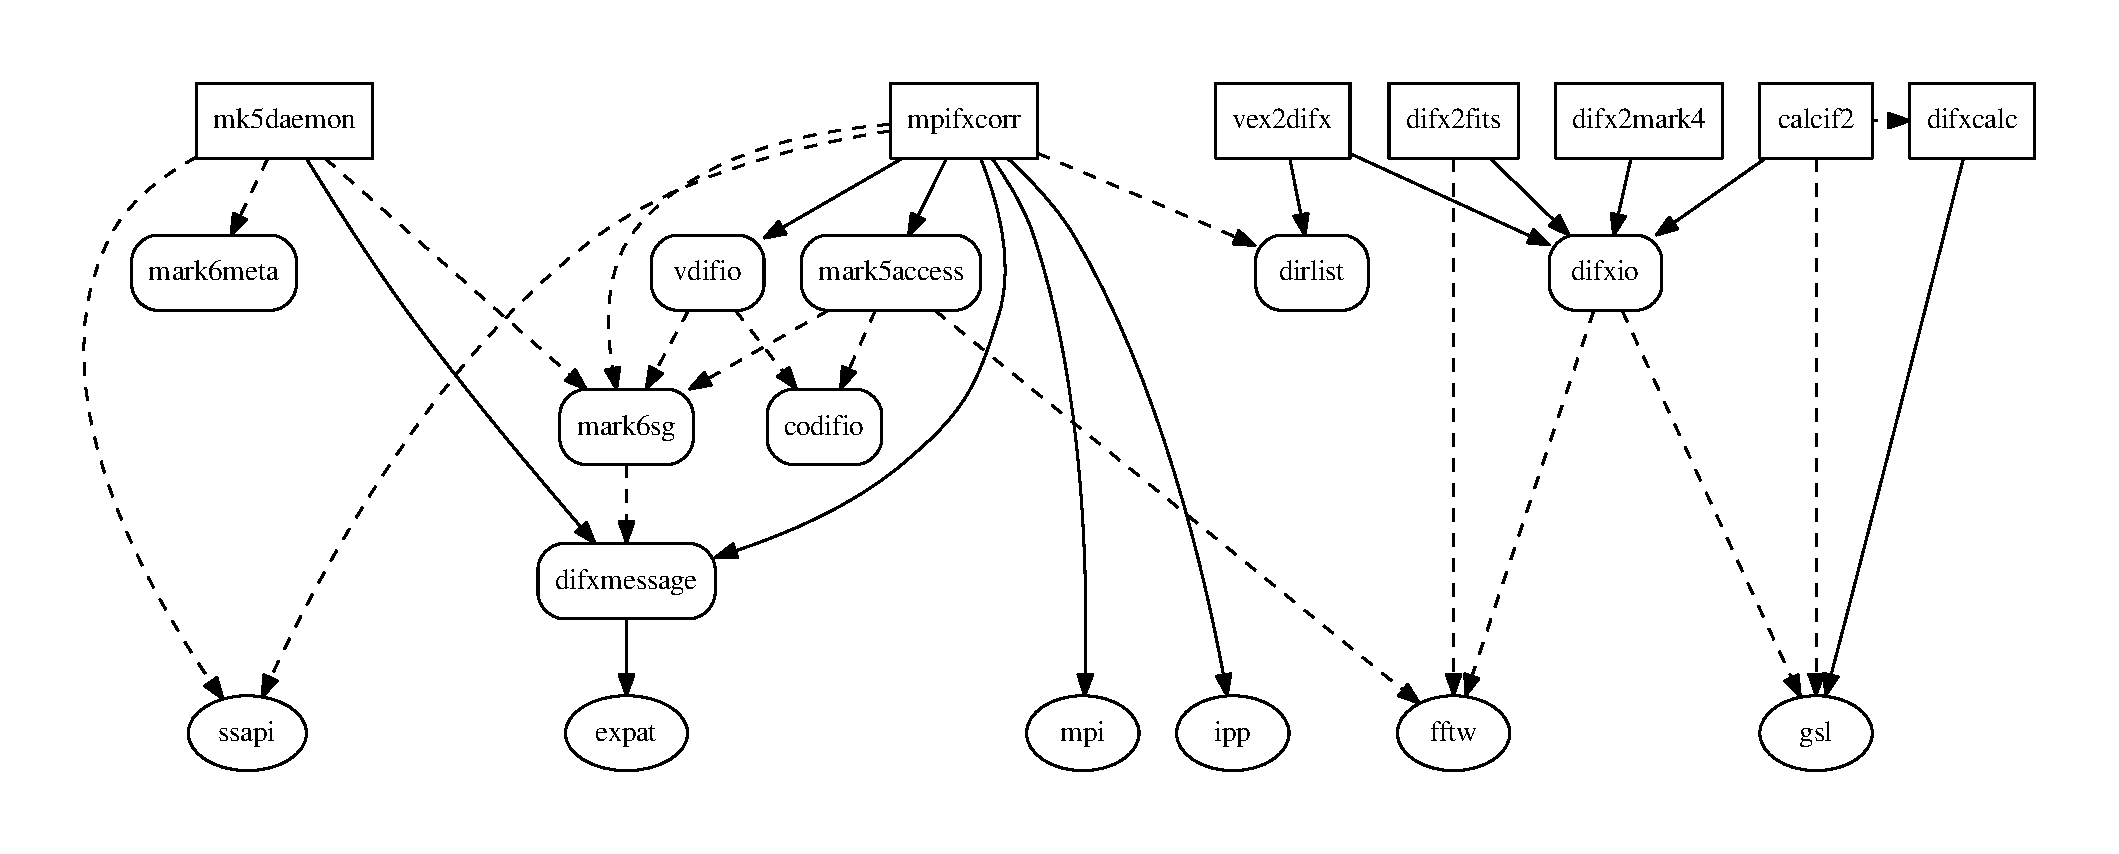
\includegraphics{difxdependency}}
\caption[dependencies]{
{\em A diagram illustrating the required and optional packages and their installation dependencies.  Rectangles inidicate applications in the DiFX suite.  Rounded rectangles are DiFX related libraries.  Ovals are third-party libraries.}
\label{fig:dependencies}
}
\end{center}
\end{figure}

The {\tt make install} steps may require root permission, depending on the {\em prefixdir} you have chosen.
If so, become root before each {\tt make install}.  
It is advisable not to compile code as root.
Be wary of errors along the way; occasional warnings may be issued, but if the building proceeds, things are probably okay.
Please report any build issues to {\tt wbrisken@nrao.edu}. 
Be warned that these instructions may change.

All of the subversion repositories below point to a {\tt difx-1.5} tagged release of the repository.
This is in order to provide a relatively stable source tree that allows development to continue on the main development branch (called {\tt trunk}).
In order to check out code that is on this development branch, simply replace {\tt tags/difx-1.5} with {\tt trunk} in all of the {\tt svn} commands below.
{\em Caveat emptor: } the {\tt trunk} branch code may at any time refuse to compile, be unstable, lack documentation, or produce incorrect results.
Don't let this stop you if you are an intrepid developer or want to see ongoing development in progress!

%If you do not have SVN access, {\tt .tar.gz} files are available from \url{http://www.aoc.nrao.edu/~wbrisken/difx-1.5/}.








% expat -----------------------------------------------------------------------

\subsubsection{expat} \label{sec:expat}

Expat is a standard library for simple XML parsing.
By default it is installed on almost all Linux distributions.
If it is not, it can be downloaded and installed based on instructions that can be found at its web page:
\url{http://expat.sourceforge.net/} .








% cx_Oracle -------------------------------------------------------------------

\subsubsection{cx\_Oracle} \label{sec:cxOracle}

In the implementation of the VLBA-DiFX operations plans, with the exception of the {\tt DOI}, all of the access to VLBA database is done using python programs that employ the cx\_Oracle library.
This library directly talks to Oracle databases; its use in Python makes for nearly effortless database interfacing.
To install:
\begin{enumerate}
\item Download the latest source distribution from \url{http://cx-oracle.sourceforge.net/} (ver.\ 5.1.2 as of this writing)
\item Decompress the contents into perhaps {\em sourcedir}; enter the newly created directory
\item Run {\tt python setup.py build}
\item Make sure install directory exists:  {\tt mkdir -p \$DIFXROOT/lib/python2.4/site-packages}
\item Run {\tt python setup.py install --prefix=\$DIFXROOT}
\end{enumerate}

\noindent
Notes:
\begin{enumerate}
\item You should substitute {\tt python2.4} with the string appropriate for your python version.
\item {\tt lib} may need to be replaced with {\tt lib64} in the path above.
\item Proper installation can be tested by running {\tt python} and typing {\tt import cx\_Oracle} at the {\tt >>>} prompt.
If another prompt is given without any ``ImportError'' message, then it should be installed properly.
\item The {\tt setup.py} file from version 5.1.2 seems to have an incompatibility with RedHat Enterprise Linux 6 (and there may be other varients of this incompatibility).
Inserting {\tt extraCompileArgs.append("-D\_\_USE\_XOPEN2K8")} at a logical outer-level location around line 200 seems to fix this problem.
\end{enumerate}






% openmpi ---------------------------------------------------------------------

\subsubsection{OpenMPI} \label{sec:mpi}

The core of DiFX uses Message Passing Interface (MPI) for inter-node communication.
Many MPI libraries exist; we choose to use OpenMPI as it is simple to install, runs well, and appears to have good community support.
\begin{enumerate}
\item Download the latest source distribution from \url{http://www.open-mpi.org/} (ver.\ 1.4.2 as of this writing)
\item Decompress the contents into perhaps {\em sourcedir}; enter the newly created directory
\item {\tt ./configure --prefix=}{\em openmpiprefix} where {\em openmpiprefix} could be the same as {\em prefixdir}, but does not have to be.
\item Run {\tt make} and finally {\tt make install} to put the parts where they belong.
\end{enumerate}








% ipp -------------------------------------------------------------------------

\subsubsection{Intel Performance Primitives} \label{sec:ipp}

Intel CPUs support an increasing variety of vector math instructions.  
The Intel Performance Primitives (IPP) makes exploiting these capabilities on any recent generation CPU simple.
An inexpensive license must be purchased to make use of these.
More information can be found on \url{http://www.intel.com}.

Once installed, set environment variable {\tt IPPROOT} to point to its install prefix, which will look something like:
{\tt /home/swc/difx/intel/ipp/6.0.2.076/ia32}; you want to choose the directory containing {\tt lib}, {\tt include}, etc.
Remember to change this in your shell initialization file as well.
This install directory should be visible to all nodes in the cluster.








% fftw ------------------------------------------------------------------------

\subsubsection{FFTW} \label{sec:fftw}

The FFTs performed by {\tt mpifxcorr} are done using the Intel Performance Primitives library, but FFTs done in an optional piece of{\tt difx2fits} and the utility {\tt m5spec} that comes with mark5access use FFTW, a standard, fast, freely available FFT library.
This library is probably installed for you with any modern Linux distribution, but you should check to make sure it is recent enough; version 3.0 and up are supported, but version 3.1.2 or newer is recommended.
If this library is not installed and the extra functionality that requires FFTW is not installed, follow the instructions below:
\begin{enumerate}
\item Download the latest source distribution from \url{http://www.fftw.org} (ver.\ 3.1.2 as of this writing)
\item Decompress the contents into perhaps {\em sourcedir}; enter the newly created directory
\item {\tt ./configure --prefix=}{\em prefixdir}
\item Run {\tt make} and finally {\tt make install} to put the parts where they belong.
\end{enumerate}








% streamstor ---------------------------------------------- INCOMPLETE --------









% difxio ----------------------------------------------------------------------

\subsubsection{difxio} \label{sec:difxio}

Parsing of text files can be tedious.  
The library difxio makes parsing difx-style files simple.
It also contains functionality to completely represent the configuration of a DiFX correlation, simplifying format conversions.
To install:
\begin{enumerate}
\item {\tt cd} {\em sourcedir}
\item Check out the subversion repository: \\
{\tt svn co }\url{https://svn.atnf.csiro.au/difx/libraries/difxio/branches/difx-1.5}{\tt\ difxio} \\
{\em Note: don't forget the {\tt difxio} at the end of the line!}
\item Enter the new directory {\tt cd difxio}
\item View the {\tt README} file.  
Note the next 5 instructions only need to be done once in this directory, even after updating the repository.
You can {\tt man} the commands if you want to know what they do.
\item {\tt aclocal}  
\item {\tt libtoolize --copy --force}
\item {\tt autoconf}
\item {\tt autoheader}
\item {\tt automake -a} 
\item Generate the Makefile: {\tt ./configure --prefix=}{\em prefixdir}
\item Build it: {\tt make}
\item Install it: {\tt make install}
\end{enumerate}

You can test for successful installation by running {\tt pkg-config --cflags difxio}.  
If you get a sensible answer, things are probably good.
If you wish to upgrade the installation:
\begin{enumerate}
\item {\tt cd} {\em sourcedir}{\tt /difxio}
\item Get updates from the repository: {\tt svn update}
\item Build it: {\tt make}
\item Install it: {\tt make install}
\end{enumerate}

Note that doing this upgrade may break other packages that depend on it, such as {\tt difx2fits} and {\tt calcif}, forcing a recompile of these programs.









% difxmessage -----------------------------------------------------------------

\subsubsection{difxmessage {\small $\mathrm{(optional)}$}} \label{sec:difxmessage}

The library difxmessage implements in the C language XML generation and parsing and multicast sending and receiving functionality that is used for communication between various parts of the DiFX system.
See \S\ref{sec:xml} for details on the XML documents supported.
The communication model is based on that of the EVLA.
This package is optional; if not built, you will not be able to use {\tt mk5daemon} or any program packaged with it, or {\tt genmachines}.
To install:
\begin{enumerate}
\item {\tt cd} {\em sourcedir}
\item Check out the subversion repository: \\
{\tt svn co }\url{https://svn.atnf.csiro.au/difx/libraries/difxmessage/branches/difx-1.5}{\tt\ difxmessage}
\item Enter the new directory {\tt cd difxmessage}
\item View the {\tt README} file.  
Note the next 5 instructions only need to be done once in this directory, even after updating the repository.
You can {\tt man} the commands if you want to know what they do.
\item {\tt aclocal}  
\item {\tt libtoolize --copy --force}
\item {\tt autoconf}
\item {\tt autoheader}
\item {\tt automake -a} 
\item Generate the Makefile: {\tt ./configure --prefix=}{\em prefixdir}
\item Build it: {\tt make}
\item Install it: {\tt make install}
\end{enumerate}

You can test for successful installation by running {\tt pkg-config --cflags difxmessage}.  
If you get a sensible answer, things are probably good.
If you wish to upgrade the installation:
\begin{enumerate}
\item {\tt cd} {\em sourcedir}{\tt /difxio}
\item Get updates from the repository: {\tt svn update}
\item Build it: {\tt make}
\item Install it: {\tt make install}
\end{enumerate}

Note that doing this upgrade may break other packages that depend on it, such as {\tt mpifxcorr} and {\tt mk5daemon}, forcing a recompile of these programs.









% mark5access -----------------------------------------------------------------

\subsubsection{mark5access} \label{sec:m5a}

mark5access is a library to parse various VLBI baseband data formats, including Mark4, VLBA, and Mark5B, with other formats to be added.
This is needed to decode these various formats from within mpifxcorr.
To install:
\begin{enumerate}
\item {\tt cd} {\em sourcedir}
\item Check out the subversion repository: \\
{\tt svn co }\url{https://svn.atnf.csiro.au/difx/libraries/mark5access/branches/difx-1.5}{\tt\ mark5access}
\item Enter the new directory {\tt cd mark5access}
\item View the {\tt README} file.  
Note the next 5 instructions only need to be done once in this directory, even after updating the repository.
\item {\tt aclocal}  
\item {\tt libtoolize --copy --force}
\item {\tt autoconf}
\item {\tt autoheader}
\item {\tt automake -a} 
\item Generate the Makefile: {\tt ./configure --prefix=}{\em prefixdir}
\item Build it: {\tt make}
\item Install it: {\tt make install}
\end{enumerate}

You can test for successful installation by running {\tt pkg-config --cflags mark5access}.  
If you get a sensible answer, things are probably good.
If you wish to upgrade the installation:
\begin{enumerate}
\item {\tt cd} {\em sourcedir}{\tt /mark5access}
\item Get updates from the repository: {\tt svn update}
\item Build it: {\tt make}
\item Install it: {\tt make install}
\end{enumerate}

Note that doing this upgrade may break other packages that depend on it, such as {\tt mpifxcorr}, forcing a recompile of these programs.









% mpifxcorr -------------------------------------------------------------------

\subsubsection{mpifxcorr}

The core of the DiFX software correlator is {\tt mpifxcorr}.  
Installation and running this program requires that MPI (\S\ref{sec:mpi}), IPP (\S\ref{sec:ipp}), difxio and mark5access all be installed.
To install:
\begin{enumerate}
\item {\tt cd} {\em sourcedir}
\item Check out the subversion repository: \\
{\tt svn co }\url{https://svn.atnf.csiro.au/difx/mpifxcorr/branches/difx-1.5}{\tt\ mpifxcorr}
\item Enter the new directory {\tt cd mpifxcorr}
\item View the {\tt README} file.  
Note the next 4 instructions only need to be done once in this directory, even after updating the repository.
\item {\tt aclocal}
\item {\tt autoconf}
\item {\tt autoheader}
\item {\tt automake -a}
\item Generate the Makefile: {\tt ./configure --prefix=}{\em prefixdir} {\tt CXX=}{\em openmpiprefix}{\tt /bin/mpicxx}
\item Build it: {\tt make}
\item Install it: {\tt make install}
\end{enumerate}

If successfully installed, the command {\tt which mpifxcorr} should return {\em prefixdir}{\tt /bin/mpifxcorr}.
If you wish to upgrade the installation:
\begin{enumerate}
\item {\tt cd} {\em sourcedir}{\tt /mpifxcorr}
\item Get updates from the repository: {\tt svn update}
\item Build it: {\tt make}
\item Install it: {\tt make install}
\end{enumerate}








% calcserver ------------------------------------------------------------------

\subsubsection{calcserver} \label{sec:calcserver}

The Goddard Space Flight Center CALC package version 9.1 is used to calculate the delay models needed for time-alignment of the raw data.
This software is wrapped in a program that exposes the capabilities of CALC via a Remote Procedure Call (RPC) and this program runs as a server.
An environment variable {\tt CALC\_SERVER} should be set that contains the name of the computer running {\tt calcserver}.
Within DiFX, the only program that makes use of this server is {\tt calcif2} (\S\ref{sec:calcif2}).
To install:
\begin{enumerate}
\item {\tt cd} {\em sourcedir}
\item Check out the subversion repository: \\
{\tt svn co }\url{https://svn.atnf.csiro.au/difx/applications/calcserver/branches/difx-1.5}{\tt\ calcserver}
\item Enter the new directory {\tt cd calcserver}
\item View the {\tt README} file.
\item {\tt aclocal}
\item {\tt libtoolize --copy --force}
\item {\tt autoconf}
\item {\tt automake -a}
\item Generate the Makefile: {\tt ./configure --prefix=}{\em prefixdir}
\item Build it: {\tt make}
\item Install it: {\tt make install}
\end{enumerate}

Since {\tt calcserver} is a single-instance program that is always running as a service, it is usually convenient to have this program start upon boot of the calcserver host.
The calcserver distribution produces a file called {\em srcDir}{\em calcserver/init.d/calcserver} that can be copied (as root) to the system {\tt /etc/init.d} directory.
After doing so, the {\tt /etc/rc.d} directories may need to be updated to run this script at the right time.
On RedHat systems, this is done with:

\noindent
{\tt /sbin/chkconfig --add calcserver}








% calcif2 ---------------------------------------------------------------------

\subsubsection{calcif2} \label{package:calcif2}

The {\tt calcif2} package contains several programs that are useful for DiFX input file creation and managing correlation, most notably {\tt calcif2} .
Note that this package used to be called {\em job2difx}.
To install:
\begin{enumerate}
\item {\tt cd} {\em sourcedir}
\item Check out the subversion repository: \\
{\tt svn co }\url{https://svn.atnf.csiro.au/difx/utilities/branches/difx-1.5/calcif2}{\tt\ calcif2}
\item Enter the new directory {\tt cd calcif2}
\item View the {\tt README} file.  
Note the next 4 instructions only need to be done once in this directory, even after updating the repository.
\item {\tt aclocal}
\item {\tt autoconf}
\item {\tt autoheader}
\item {\tt automake -a}
\item Generate the Makefile: {\tt ./configure --prefix=}{\em prefixdir}
\item Build it: {\tt make}
\item Install it: {\tt make install}
\end{enumerate}

If successfully installed, the command {\tt which calcif2} should return {\em prefixdir}{\tt /bin/calcif2}.
Several other programs should also be installed, including: {\tt genmachines}, {\tt getjobs}, {\tt jobdisks}, {\tt joblist}, {\tt jobstatus}, {\tt difxsniff}, {\tt mk5take}, {\tt mk5return}, and {\tt vlog}.
If you wish to upgrade the installation:
\begin{enumerate}
\item {\tt cd} {\em sourcedir}{\tt /calcif2}
\item Get updates from the repository: {\tt svn update}
\item Build it: {\tt make}
\item Install it: {\tt make install}
\end{enumerate}







% difx2fits -------------------------------------------------------------------

\subsubsection{difx2fits}

The initial NRAO adaptation of DiFX is designed to interface as seamlessly as possible into our existing infrastructure and habits.
This means generation of FITS-IDI output files for compliance with AIPS.
The program {\tt difx2fits} takes many input files (see Fig.~\ref{fig:block}) and produces a FITS file for every DiFX input file.
To install:
\begin{enumerate}
\item {\tt cd} {\em sourcedir}
\item Check out the subversion repository: \\
{\tt svn co }\url{https://svn.atnf.csiro.au/difx/applications/difx2fits/branches/difx-1.5}{\tt\ difx2fits}
\item Enter the new directory {\tt cd difx2fits}
\item View the {\tt README} file.  
Note the next 4 instructions only need to be done once in this directory, even after updating the repository.
\item {\tt aclocal}
\item {\tt autoconf}
\item {\tt autoheader}
\item {\tt automake -a}
\item Generate the Makefile: {\tt ./configure --prefix=}{\em prefixdir}
\item Build it: {\tt make}
\item Install it: {\tt make install}
\end{enumerate}

If successfully installed, the command {\tt which difx2fits} should return {\em prefixdir}{\tt /bin/difx2fits}.
If you wish to upgrade the installation:
\begin{enumerate}
\item {\tt cd} {\em sourcedir}{\tt /difx2fits}
\item Get updates from the repository: {\tt svn update}
\item Build it: {\tt make}
\item Install it: {\tt make install}
\end{enumerate}








% mk5daemon -------------------------------------------------------------------

\subsubsection{mk5daemon {\small $\mathrm{(optional)}$}} 

The optional package {\tt mk5daemon} relies on package {\tt difxmessage} and is only really needed for installations requiring playback off Mark5 modules.
Root permission is required for proper installation and running of this program.
See \S\ref{sec:mk5daemon} for a description of the main program, {\tt mk5daemon}, that comes with this package.
Other useful scripts are included here.
To install:
\begin{enumerate}
\item {\tt cd} {\em sourcedir}
\item Check out the subversion repository: \\
{\tt svn co }\url{https://svn.atnf.csiro.au/difx/applications/mk5daemon/branches/difx-1.5}{\tt\ mk5daemon}
\item Enter the new directory {\tt cd mk5daemon}
\item View the {\tt README} file.  
Note the next 4 instructions only need to be done once in this directory, even after updating the repository.
\item {\tt aclocal}
\item {\tt autoconf}
\item {\tt autoheader}
\item {\tt automake -a}
\item Generate the Makefile: {\tt ./configure --prefix=}{\em prefixdir}
\item Build it: {\tt make}
\item Install it: {\tt make install}
\item Ensure that this program starts at boot.
This requires the following to occur on each computer in the cluster.
Note that the instructions may vary depending on your operating system.
The program is likely to get started before NSF is started, so {\tt mk5daemon} should be installed locally on each compute in the cluster.
On each machine, run as root: {\tt cp }{\em prefixdir}{\tt /bin/mk5daemon} {\em localdir} {\tt ; echo }{\em localdir}{\tt /mk5daemon >> /etc/rc.local} .
Here {\em localdir} is a directory on the particular machine, such as {\tt /usr/bin}
This only needs to be run
\end{enumerate}

If successfully installed, the command {\tt which mk5daemon} should return {\em prefixdir}{\tt /bin/mk5daemon}.
If you wish to upgrade the installation:
\begin{enumerate}
\item {\tt cd} {\em sourcedir}{\tt /mk5daemon}
\item Get updates from the repository: {\tt svn update}
\item Build it: {\tt make}
\item Install it: {\tt make install}
\item Copy it to the local disk (as root): {\tt cp -f }{\em prefixdir}{\tt /bin/mk5daemon} {\em localdir}
\end{enumerate}








% vex2difx --------------------------------------------------------------------

\subsubsection{vex2difx}

The {\tt vex2difx} program aims to convert any legal, complete vex format experiment description file into {\tt .input} and {\tt .calc} files for use with DiFX.
To install:
\begin{enumerate}
\item {\tt cd} {\em sourcedir}
\item Check out the subversion repository: \\
{\tt svn co }\url{https://svn.atnf.csiro.au/difx/applications/vex2difx/branches/difx-1.5}{\tt\ vex2difx}
\item Enter the new directory {\tt cd vex2difx}
\item View the {\tt README} file.  
Note the next 4 instructions only need to be done once in this directory, even after updating the repository.
\item {\tt aclocal}
\item {\tt autoconf}
\item {\tt autoheader}
\item {\tt automake -a}
\item Generate the Makefile: {\tt ./configure --prefix=}{\em prefixdir}
\item Build it: {\tt make}
\item Install it: {\tt make install}
\end{enumerate}

If successfully installed, the command {\tt which vex2difx} should return {\em prefixdir}{\tt /bin/vex2difx}.
If you wish to upgrade the installation:
\begin{enumerate}
\item {\tt cd} {\em sourcedir}{\tt /vex2difx}
\item Get updates from the repository: {\tt svn update}
\item Build it: {\tt make}
\item Install it: {\tt make install}
\end{enumerate}









% difx_db ------------------------------------------------- NRAO ONLY ---------

\subsubsection{difx\_db {\small $\mathrm{(NRAO\ only)}$}}

Package {\tt difx\_db} contains several scripts that either make direct connection to the VLBA database or require site-specific access.
Thus, this package is not available from the standard DiFX repositories.
If any programs in this package seem especially appropriate for use at a correlator other than the VLBA DiFX correlator, please let me know and I'll see what I can do to make it more generally useful.
To install:
\begin{enumerate}
\item {\tt cd} {\em sourcedir}
\item Check out the subversion repository
\item Enter the new directory {\tt cd difx\_db}
\item View the {\tt README} file.  
Note the next 4 instructions only need to be done once in this directory, even after updating the repository.
\item {\tt aclocal}
\item {\tt autoconf}
\item {\tt automake -a}
\item Generate the Makefile: {\tt ./configure --prefix=}{\em prefixdir}
\item Build it: {\tt make}
\item Install it: {\tt make install}
\item ({\em as root}) Change file ownership: {\tt chown root} {\em prefixdir}{\tt /e2ecopy}
\item ({\em as root}) Set UID: {\tt chmod +s} {\em prefixdir}{\tt /e2ecopy}
\end{enumerate}

If successfully installed, the command {\tt which difxqueue} should return {\em prefixdir}{\tt /bin/difxqueue}.
If you wish to upgrade the installation:
\begin{enumerate}
\item {\tt cd} {\em sourcedir}{\tt /vex2difx}
\item Get updates from the repository: {\tt svn update}
\item Build it: {\tt make}
\item Install it: {\tt make install}
\item ({\em as root}) Change file ownership: {\tt chown root} {\em prefixdir}{\tt /e2ecopy}
\item ({\em as root}) Set UID: {\tt chmod +s} {\em prefixdir}{\tt /e2ecopy}
\end{enumerate}
